\documentclass{beamer}
\usepackage[utf8x]{inputenc}
%\usepackage[latin1]{inputenc}
\usepackage[ngerman]{babel}
\usepackage{graphicx}
\usetheme{Warsaw}
\usecolortheme{default}
\useinnertheme{circles}
%\useoutertheme{smoothbars}
%\useoutertheme{infolines}
%\useoutertheme{miniframes}
%\useoutertheme{sidebar}
%\useoutertheme{split}
%\useoutertheme{shadow}
%\useoutertheme{smoothtree}
%\useoutertheme{tree}
%\useoutertheme{miniframes}
\usepackage{amsmath}
\usepackage{amsfonts}
\usepackage{amssymb}
\setbeamercovered{transparent}
\title{Architekturen in Java - Java Server Faces}
\author{Urban - Cuartas}
\institute[]{Hochschule Augsburg}
%\logo{\pgfimage[width=2cm,height=2cm]{bilder/logo.jpg}}
\date{\today}

\begin{document}
\frame{\titlepage}
\section[]{}
\frame{
	\frametitle{Inhaltsverzeichnis}
	\begin{columns}[c]
	\begin{column}{5cm}
		\tableofcontents[section, subsectionstyle=hide]
	\end{column}
	\begin{column}{5cm}
		\begin{figure}[htbp]
 		 \centering
%			\includegraphics[width=5cm,height=4cm]{bilder/inhaltsverzeichnis.jpg}
		\end{figure}
	\end{column}
	\end{columns}
}

\section{Einführung}
\frame{
	\frametitle{Was sind JSFs?}
		\begin{columns}[c]
		\begin{column}{5cm}
        \begin{block}{Beschreibung}
			\begin{itemize}
				\item Spezifikation von Sun 
				\item Vorteile für Webentwickler, Java Programmierer, Tool-Hersteller
				\item Verschiedene Implementierungen 			
				\item Erstellung von Web-UIs
				\item Nutzt MVC  
            \end{itemize}
        \end{block}
		\end{column}
		\begin{column}{5cm}
			\begin{figure}[htbp]
 			 \centering
				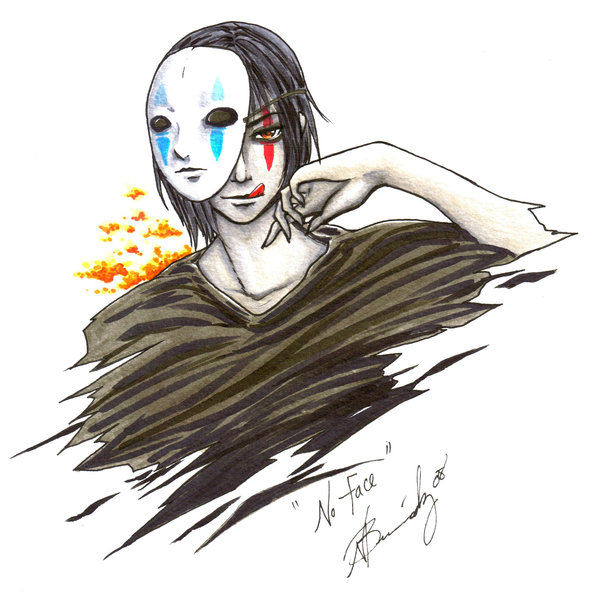
\includegraphics[width=4cm,height=3cm]{bilder/faces.jpg}
			  \caption{jsf}
			  \label{JSF}
			\end{figure}

		\end{column}

		\end{columns}
}

\frame{
	\frametitle{Implementierungen}
		\begin{columns}[c]
		\begin{column}{5cm}
        \begin{block}{Beschreibung}
			\begin{itemize}
				\item Mojarra (Sun) 
				\item MyFaces (Apache)
				\item ICEFaces (Ajax erweiterung) 
            \end{itemize}
        \end{block}
		\end{column}
		\begin{column}{5cm}
			\begin{figure}[htbp]
 			 \centering
				
\includegraphics[width=4cm,height=3cm]{bilder/MyFaces_logo.jpg}
			  \caption{implementierung}
			  \label{Implementierung}
			\end{figure}

		\end{column}

		\end{columns}
}
\frame{
	\frametitle{Vorteile}
		\begin{columns}[c]
		\begin{column}{5cm}
        \begin{block}{Beschreibung}
			\begin{itemize}
				\item Trennung zwischen Darstellung und Geschäftslogik
				\item Einfaches erstellen von UI Komponenten 
				\item Keine Festlegung auf den View-Handler (JSP, Facelets) 
				\item Projektentwicklung kann parallelisiert werden
				\item Responsecode kann z.B. HTML oder WML sein
            \end{itemize}
        \end{block}
		\end{column}
		\begin{column}{5cm}
			\begin{figure}[htbp]
 			 \centering
				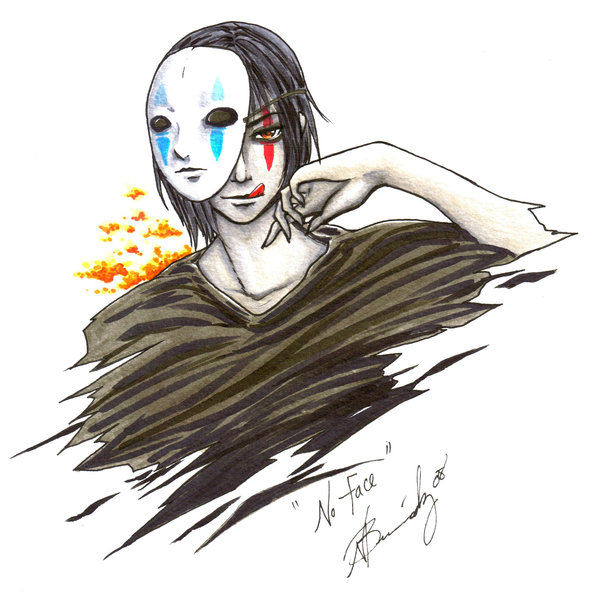
\includegraphics[width=4cm,height=3cm]{bilder/faces.jpg}
			  \caption{jsf}
			  \label{JSF}
			\end{figure}

		\end{column}

		\end{columns}
}

\frame{
	\frametitle{Beispiel-Sicht}
	\begin{figure}[htbp]
 			 \centering
				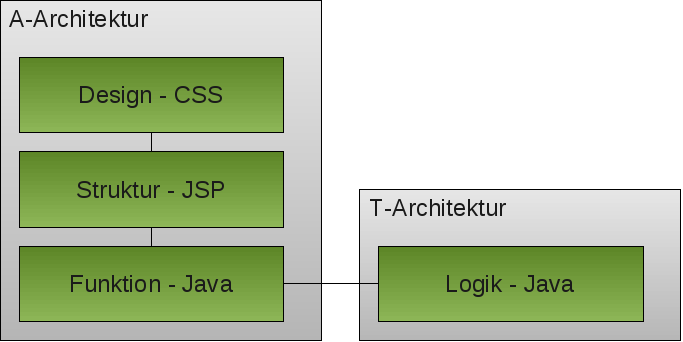
\includegraphics[width=10cm,height=4cm]{bilder/Sichten.png}
			  \caption{Beispiel-Sicht}
			  \label{sicht}
	\end{figure}
}

\frame{
	\frametitle{Facelets}
		\begin{columns}[c]
		\begin{column}{5cm}
        \begin{block}{Beschreibung}
			\begin{itemize}
				\item Setzt gültige XML-Dokumente voraus  
				\item Component Aliasing 
				\item Suffix normalerweise *.xhtml 
				\item Eingeschränkte JSTL Unterstützung 
				\item Unabhängig von einem JSP Container 
            \end{itemize}
        \end{block}
		\end{column}
		\begin{column}{5cm}
			\begin{figure}[htbp]
 			 \centering
				
\includegraphics[width=4cm,height=5cm]{bilder/facelets.jpg}
			  \caption{Facelets}
			  \label{facelets}
			\end{figure}

		\end{column}

		\end{columns}
}

\frame{
	\frametitle{MVC und JSF}
		\begin{figure}[htbp]
 			 \centering
				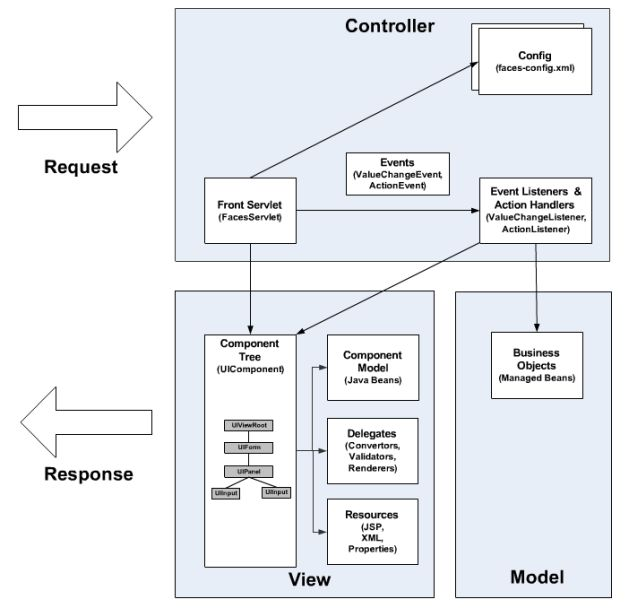
\includegraphics[width=8cm,height=6cm]{bilder/mvcJSF.jpg}
			  \caption{MVC}
			  \label{mvc}
		\end{figure}

}

\frame{
	\frametitle{JSF und Applikations-Frameworks wie Struts}
		\begin{columns}[c]
		\begin{column}{5cm}
        \begin{block}{Beschreibung}
			\begin{itemize}
				\item JSF kann mit Struts kombiniert werden 
				\item Struts als Applikationsframework 
				\item und JSF als UI-Framework 
            \end{itemize}
        \end{block}
		\end{column}
		\begin{column}{5cm}
			\begin{figure}[htbp]
 			 \centering
				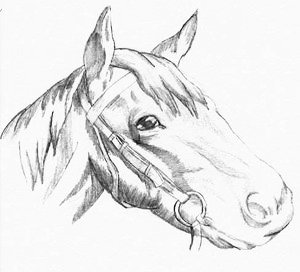
\includegraphics[width=4cm,height=3cm]{bilder/struts.jpg}
			  \caption{Struts}
			  \label{struts}
			\end{figure}

		\end{column}

		\end{columns}
}


\frame{
	\frametitle{Zusammenhang zwischen Servlets, JSP und JSF}
		\begin{columns}[c]
		\begin{column}{5cm}
        \begin{block}{Beschreibung}
			\begin{itemize}
				\item Basis: Servlets für Request und Response
				\item Als View kann JSP mit JSF benutzwerden 
				\item Aber auch JSF mit Facelets realisiert werden 
            \end{itemize}
        \end{block}
		\end{column}
		\begin{column}{5cm}
			\begin{figure}[htbp]
 			 \centering
				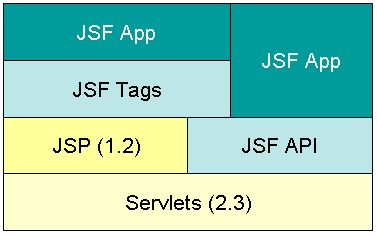
\includegraphics[width=4cm,height=3cm]{bilder/jsfJspServletsZusammenhang.jpg}
			  \caption{Zusammenhang}
			  \label{zusammenhang}
			\end{figure}

		\end{column}
		\end{columns}
}
\frame{
	\frametitle{JSF Lifecycle}
			\begin{figure}[htbp]
 			 \centering
				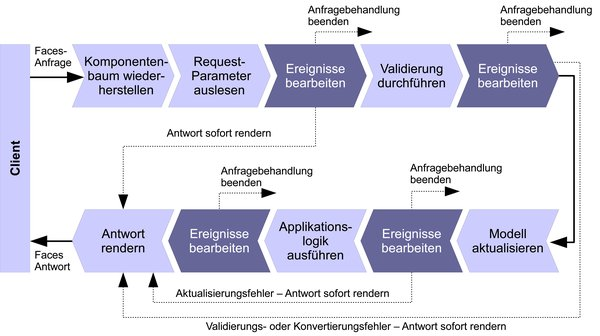
\includegraphics[width=8cm,height=6cm]{bilder/lifecycle-complete-de.jpg}
			  \caption{JSF Lifecycle}
			  \label{lifecycle}
			\end{figure}
}

\frame{
	\frametitle{Event-Handling}
		\begin{columns}[c]
		\begin{column}{5cm}
        \begin{block}{Action Event}
			\begin{itemize}
				\item  Wird in der Request Parameter auslesen-Phase generiert
				\item  Aber erst in der Applikationslogik ausführen-Phase an den Listener übergeben
				\item action bzw. actionListner-Attribut oder actionListener-Tag
            \end{itemize}
        \end{block}
		\end{column}
		\begin{column}{5cm}
			\begin{figure}[htbp]
 			 \centering
				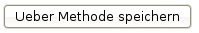
\includegraphics[width=4cm,height=1cm]{bilder/button.jpg}
			  \caption{Action Event}
			  \label{actionEvent}
			\end{figure}

		\end{column}
		\end{columns}
}

\frame{
	\frametitle{Event-Handling}
		\begin{columns}[c]
		\begin{column}{5cm}
        \begin{block}{Value-Change Event }
			\begin{itemize}
				\item Wenn sich ein Wert im Model ändert (Modell aktualisieren Phase)
				\item valueChangeListener-Attribut
				\item valueChangeListener-Tag
            \end{itemize}
        \end{block}
		\end{column}
		\begin{column}{5cm}
			\begin{figure}[htbp]
 			 \centering
				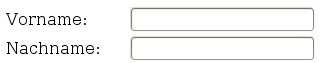
\includegraphics[width=4cm,height=2cm]{bilder/form.jpg}
			  \caption{Value-Change Event}
			  \label{valueChangeEvent}
			\end{figure}

		\end{column}
		\end{columns}
}

\frame{
	\frametitle{Event-Handling}
		\begin{columns}[c]
		\begin{column}{5cm}
        \begin{block}{Phase Event}
			\begin{itemize}
				\item Kann zur einer oder zu allen Phasen aufgerufen werden
				\item Alle Phasen zu überwachen eignet sich vor allem zum Debuging, Monitoring oder Logging
				\item Eine einzelne Phase zu überwachen ist z.B. beim Überprüfen eines Logins sinnvoll
            \end{itemize}
        \end{block}
		\end{column}
		\begin{column}{5cm}
			\begin{figure}[htbp]
 			 \centering
				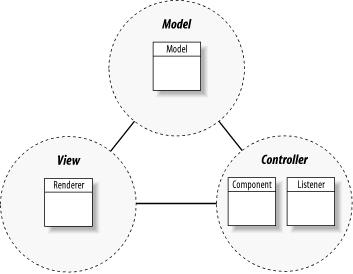
\includegraphics[width=4cm,height=3cm]{bilder/mvc.jpg}
			  \caption{Phase Event}
			  \label{phaseEvent}
			\end{figure}

		\end{column}
		\end{columns}
}

\section{Vorbereitung}

\frame{
	\frametitle{Benötigte Software}
		\begin{columns}[c]
		\begin{column}{5cm}
        \begin{block}{Beschreibung}
			\begin{itemize}
				\item ServletContainer z.B. Tomcat  
				\item JSP Standard Tag Library (JSTL), um die JSF Taglibraries einzubinden
				\item JSF Implementierung z.B. Mojarra 
            \end{itemize}
        \end{block}
		\end{column}
		\begin{column}{5cm}
			\begin{figure}[htbp]
 			 \centering
				
\includegraphics[width=4cm,height=3cm]{bilder/tomcat10.jpg}
			  \caption{Container}
			  \label{container}
			\end{figure}

		\end{column}
		\end{columns}
}

\frame{
	\frametitle{Demo1}\begin{figure}[htbp]
 			 \centering
				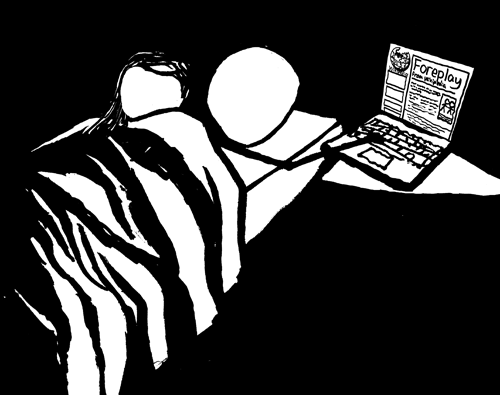
\includegraphics[width=8cm,height=6cm]{bilder/getting_out_of_hand.png}
			  \caption{Demo1}
			  \label{demo1}
			\end{figure}
}

\frame{
	\frametitle{ICEfaces}
		\begin{columns}[c]
		\begin{column}{5cm}
        \begin{block}{Beschreibung}
			\begin{itemize}
				\item RIA mit Ajax  
				\item JavaScript-Code zur Laufzeit erzeugt
				\item nahtlos zu Java EE kompatibel
            \end{itemize}
        \end{block}
		\end{column}
		\begin{column}{5cm}
			\begin{figure}[htbp]
 			 \centering
				
\includegraphics[width=3cm,height=2cm]{bilder/icefaces.png}
			  \caption{ICEfaces}
			  \label{icefaces}
			\end{figure}

		\end{column}
		\end{columns}
}

\section{ICEfaces}

\frame{
	\frametitle{AJAX}\begin{figure}[htbp]
 			 \centering
				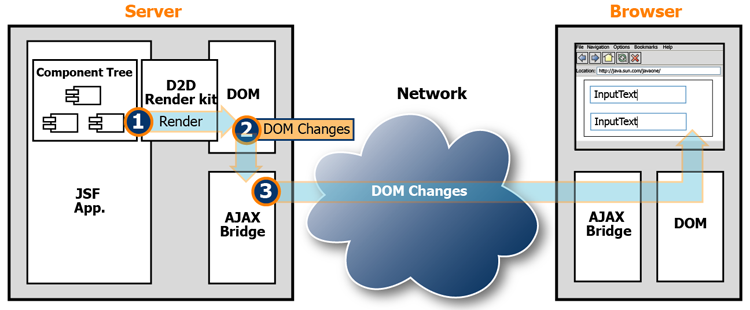
\includegraphics[width=10cm,height=4cm]{bilder/ICEfaces-Direct-to-DOM.png}
			  \caption{AJAX}
			  \label{ajax}
			\end{figure}
}

\frame{
	\frametitle{Drag and Drop}\begin{figure}[htbp]
 			 \centering
				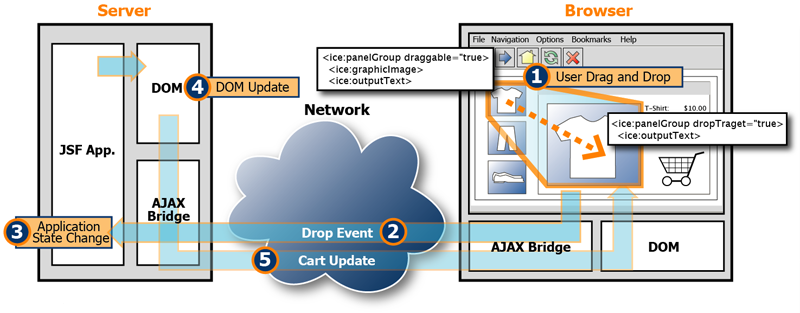
\includegraphics[width=10cm,height=4cm]{bilder/ICEfaces-Drag-an-Drop.png}
			  \caption{Drag and Drop}
			  \label{dragndrop}
			\end{figure}
}
\end{document}
